%% DESIGN: Montserrat | Futuristic gradient header (tikz) | Electric purple (#9B30FF) accent
\documentclass[11pt,a4paper]{article}
\usepackage[left=0.6in,right=0.6in,top=0.3in,bottom=0.5in]{geometry}
\usepackage[T1]{fontenc}
\usepackage[defaultfam,tabular,lining]{montserrat}
\usepackage{xcolor,titlesec,enumitem,hyperref,tikz}

\definecolor{accent}{HTML}{9B30FF}
\definecolor{ACCENT}{HTML}{9B30FF}
\definecolor{accent2}{HTML}{4B0082}
\definecolor{glow}{HTML}{E8D5FF}
\hypersetup{colorlinks=true,urlcolor=accent}
\pagestyle{empty}

\titleformat{\section}{\normalsize\bfseries\uppercase}{}{0em}{\colorbox{glow}{\color{accent2}\,#1\,}}[]
\titlespacing{\section}{0pt}{1em}{0.4em}

\begin{document}

% Futuristic gradient header
\noindent

\begin{tikzpicture}[remember picture]
\shade[left color=accent2,right color=accent] (0,0) rectangle (\textwidth,2.8);
% Decorative circles
\foreach \x/\r/\o in {2/0.8/0.05, 4/0.5/0.08, 13/1.0/0.04, 15/0.6/0.06} {
  \fill[white,opacity=\o] (\x,1.4) circle (\r);
}
% Grid lines
\foreach \y in {0.5,1.0,...,2.5} {
  \draw[white,opacity=0.05] (0,\y) -- (\textwidth,\y);
}
\node[anchor=west,text=white,font=\Huge\bfseries] at (0.4,1.9) {KAI RODRIGUEZ};
\node[anchor=west,text=white!90,font=\large] at (0.4,1.1) {Generative AI Engineer};
\node[anchor=west,text=white!75,font=\small] at (0.4,0.4) {kai.rodriguez@email.com \quad\textbar\quad (555) 012-3456 \quad\textbar\quad San Francisco, CA \quad\textbar\quad github.com/kaigen};
\end{tikzpicture}

\vspace{0.6em}

\section{About}
GenAI Engineer at the frontier of large language models and generative systems. 4+ years building production AI applications including chatbots, code generation tools, and creative AI systems. Deep expertise in prompt engineering, fine-tuning, and RLHF.

\section{Core Technologies}
\noindent
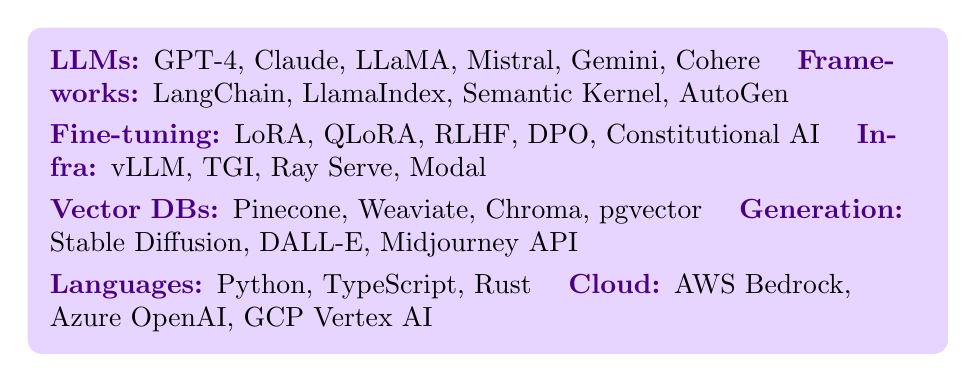
\begin{tikzpicture}
\node[fill=glow,rounded corners=5pt,inner sep=8pt,text width=\textwidth-1cm] {
\textbf{\color{accent2}LLMs:} GPT-4, Claude, LLaMA, Mistral, Gemini, Cohere \quad
\textbf{\color{accent2}Frameworks:} LangChain, LlamaIndex, Semantic Kernel, AutoGen\\[3pt]
\textbf{\color{accent2}Fine-tuning:} LoRA, QLoRA, RLHF, DPO, Constitutional AI \quad
\textbf{\color{accent2}Infra:} vLLM, TGI, Ray Serve, Modal\\[3pt]
\textbf{\color{accent2}Vector DBs:} Pinecone, Weaviate, Chroma, pgvector \quad
\textbf{\color{accent2}Generation:} Stable Diffusion, DALL-E, Midjourney API\\[3pt]
\textbf{\color{accent2}Languages:} Python, TypeScript, Rust \quad
\textbf{\color{accent2}Cloud:} AWS Bedrock, Azure OpenAI, GCP Vertex AI
};
\end{tikzpicture}

\section{Experience}

\noindent\textbf{Senior GenAI Engineer} \hfill \textcolor{accent}{Jan 2023 -- Present}\\
\textit{FutureAI Labs, San Francisco, CA}
\begin{itemize}[leftmargin=1.2em,nosep,label={\color{accent}$\star$}]
\item Architected multi-agent AI system handling complex reasoning tasks (30\% improvement over single-agent)
\item Built enterprise RAG platform with hybrid search, reranking, and citation generation (95\% accuracy)
\item Implemented RLHF pipeline for custom LLM alignment, reducing harmful outputs by 90\%
\item Designed prompt optimization framework automating prompt engineering (2x developer productivity)
\item Led evaluation infrastructure: automated benchmarks, human eval pipelines, red-teaming
\end{itemize}
\vspace{0.5em}

\noindent\textbf{ML Engineer -- NLP/GenAI} \hfill \textcolor{accent}{Jun 2021 -- Dec 2022}\\
\textit{ConversAI, Palo Alto, CA}
\begin{itemize}[leftmargin=1.2em,nosep,label={\color{accent}$\star$}]
\item Built conversational AI platform serving 5M+ monthly users with GPT-based dialogue
\item Fine-tuned domain-specific models for legal and medical Q\&A (40\% better than base models)
\item Implemented streaming inference reducing perceived latency by 70\%
\item Created content moderation pipeline using LLM-as-judge pattern
\end{itemize}
\vspace{0.5em}

\noindent\textbf{Software Engineer -- AI} \hfill \textcolor{accent}{Aug 2019 -- May 2021}\\
\textit{CodeAssist Inc., Seattle, WA}
\begin{itemize}[leftmargin=1.2em,nosep,label={\color{accent}$\star$}]
\item Developed code generation tool using fine-tuned Codex models (adopted by 10K+ developers)
\item Built automated code review system using LLMs for style and bug detection
\end{itemize}

\section{Education}
\noindent\textbf{M.S. Artificial Intelligence} \hfill Stanford University, 2019 \qquad \textbf{B.S. CS} \hfill MIT, 2017

\end{document}
